\chapter{Conclusions and Future Work}
\label{Chapter-Conclusions}
\lhead{Chapter 6. \emph{Conclusions and Future Work}}

\section{Scope of Thesis}%
\label{sec:scope_of_thesis}

%Motivation
% From universalities abstract
The importance of the network architecture for the mechanical properties of biopolymer networks is often obscured by focussing on the properties of single-components. \cite{storm_nonlinear_2005}, demonstrated that the nonlinear response of a strained network can be explained taking into account the non-linear properties of single-biopolymer and assuming that the network architecture is isotropic and homogeneous. This bottom-up approach has proven successful for a wide range of biopolymers \cite{carrillo_nonlinear_2013}, but might not be enough to explain the detailed onset of strain-stiffening and the exponent of the non-linear response, as shown recently with other protein networks\cite{licup_stress_2015}. An alternative explanation to non-linear elasticity was given with the focus on network architecture in the material\cite{onck_alternative_2005}, pointing out that the fine-grain control of non-linear elasticity depended on single-biopolymer components, \textbf{the linkage characteristics}, and \textbf{the geometry of the connections}.

% In order to study and compare different network geometries, a graph representation of the network is suitable, taking advantage of methods utilized in the field of complex networks. With this approach we could also explore the mechanisms of network formation,
% and see if there are connections between similar statistical distributions of the graph and the similarities showed by protein and polysaccharide networks \cite{carrillo_nonlinear_2013}.

Non-affine deformations are at the core of explaining the complex behaviour of biopolymer networks, but methods to reliably gather the geometry of the networks have been lacking and are the focus of this thesis. Affine regimes have been shown to be capable in characterizing the mechanical properties of bulk and dense materials, but in biology this is not always the case.

\section{Summary}%
\label{sec:conclusions_summary}

%Chapter Wavelets/image-tools
I rely on 3D imaging, tomography or Z stacks of images, to extract the network geometry more reliably than would be possible from 2D images. I provided tools for image analysis in 3D in a high-performance computing language, and contributed them, fully tested and documented to the de-facto standard image analysis library ITK (\autoref{Chapter-Wavelets}).

% Chapter TEM-SAXS
Gathering the network structure from images requires that the information extracted is reliable. In \autoref{Chapter-TEMSAXS} several distinct polysaccharide gels networks were realized. A set of these networks was further treated for study by transmission electron microscopy (TEM), which requires additional preparation. Another set of the same networks, this time unadulterated, was studied by small-angle x-ray scattering (SAXS). The comparison between the two techniques showed that careful protocols can produce datasets where information acquired by imaging above around 20 nm is broadly consistent with that obtained by SAXS studies carried out on unadulterated samples.
The fact that at larger length scales the structure of the networks is preserved in the TEM samples, allow us to extract and quantify the network architecture and connectivity with confidence, information that is lost in scattering experiments owing to the intrinsic averaging nature of the technique.

% Chapter Image / Extraction
I pursued the task of extracting the network architectures from images in \autoref{Chapter-Image} using a pipeline of image analysis to denoise and binarize the original images. I then developed state-of-the-art algorithms taken from the digital topology community to skeletonize the image, being aware of not changing the topology of the original network in the process. With a thin-image and introducing novel tools in this area, I created a one-to-one map between the image and a spatial graph, connecting in this way the image analysis field with the area of complex networks. I am now capable of studying and characterizing our networks of biopolymers with a wider range of tools.

I computed the degree, end-to-end node distances, contour lengths, angle, and direction cosines of those angles to characterize our sample networks of different biopolymers, ranging from actin filaments, to polysaccharides, such as pectin and carrageenan. The statistical distributions of these properties show strong similarities between protein and polysaccharides networks. Such universalities should be further explored to understand their origin.

% Chapter Reconstruction
I also provided a simulated annealing tool in \autoref{Chapter-Reconstruction} to recreate networks completely in-silico given a set of statistical distributions: degree, end-to-end distance, and director cosines. This allows the theoretical exploration of networks in-silico just changing the input distributions. Future work in this area might include adding distributions for other graph properties for finer control.

\section{Conclusions}%
\label{sub:conclusions_conclusions}

I have focused in bringing computation tools to the community (all the work is open source, tested and documented) where we can start investigating low density, non-affine networks from a more analytical point of view, I foresee theoreticians and modellers taking these networks \textbf{extracted from experimental results} as starting points for their models, instead of relying on the more homogeneous mikado model, and providing a greater scale approach than lattice models.

\begin{itemize}[topsep=0pt]
  \item Validated transmission electron microscopy (TEM) imaging as a reliable tool to examine polysaccharides network geometries after its comparison with small-angle x-ray scattering.
  \item Provided a mapping between images and spatial graphs, allowing the study of these networks with the tools from the complex systems and networks field.
  \item Found universalities of certain graph properties in the geometry of gel-like biopolymer networks at different scales.
  \item Provided a tool to reconstruct networks in-silico based on statistical distribution. This allows the exploration of different network architectures that can be used in modelling and simulating behaviour of these networks under different conditions.
\end{itemize}

\begin{figure}[H]
  \begin{center}
    \begin{tikzpicture}[scale=0.8]
      \node[blockimage] (A) at (2,8.5) {
      \textsc{Image Analysis}};
      \node[blocknetwork] (B) at (8.5,3) {%
        \begin{center}
        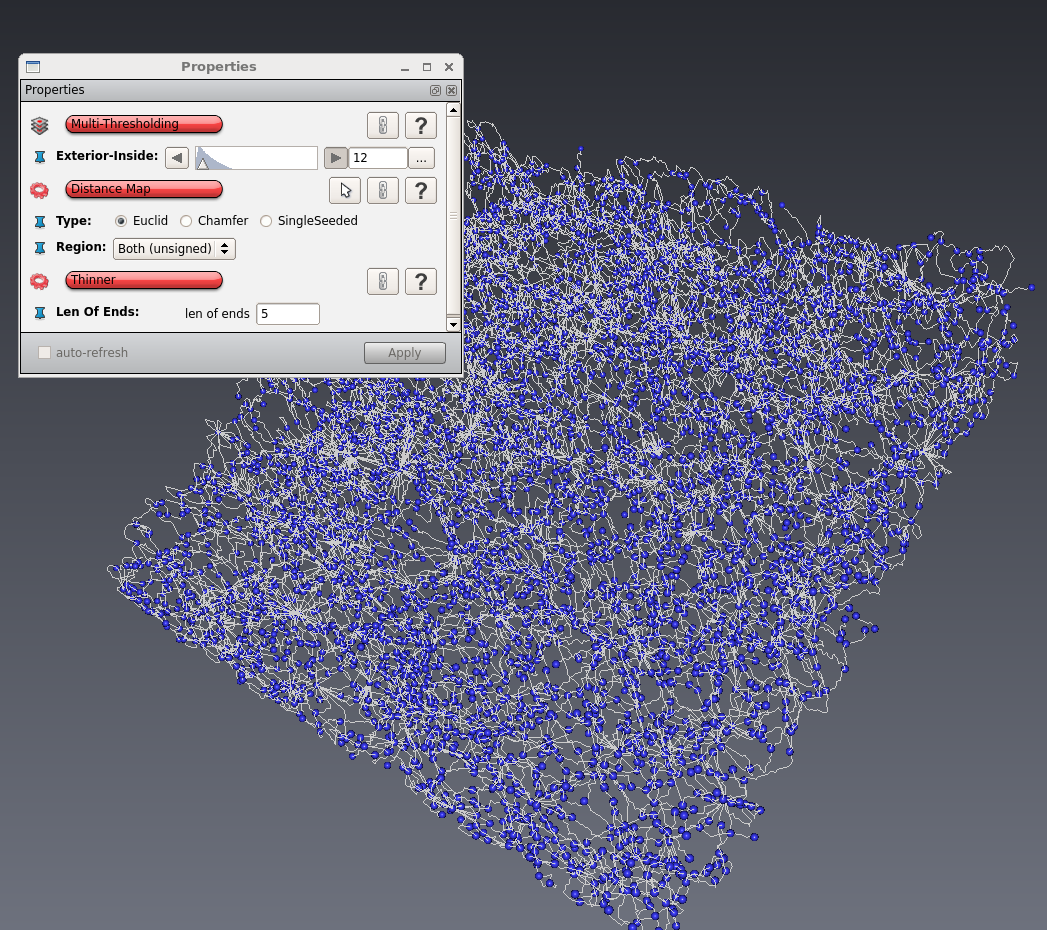
\includegraphics[width=1.0\textwidth]{Figures/chapter-image/avizo/ActinAllan11jun132_BIN12LEN5.png}%
        \end{center}

       \textsc{Network /}\\
       \textsc{Spatial Graph}
        };

      \node[blockimage] (C) at (1.5,0) {
      \textsc{Reconstruction}\\
      \textsc{Algorithm}
      };
      \node[blocknetwork] (F) at (0,3.5) {
      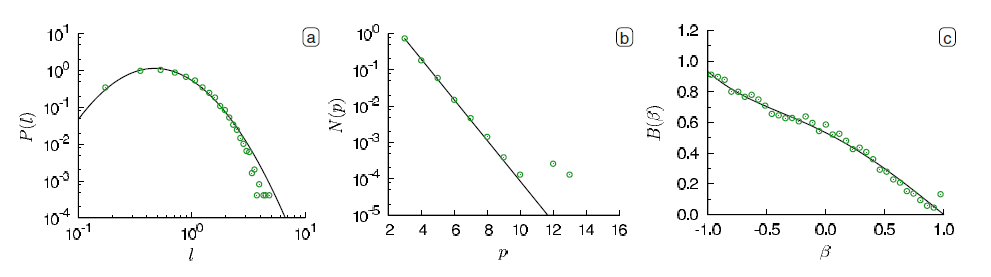
\includegraphics[width=1.0\textwidth]{Figures/chapter-reconstruct/lindstrom-paper-images.png}%

      \textsc{Statistics}
      };

      \node[blockmodel] (D) at (15,3) {\textsc{Modeling}};

      \draw[green,arrows={-triangle 45}] (A) -- (B);
      \draw[blue,arrows={-triangle 45}] (B) -- (F);
      \draw[blue,arrows={-triangle 45}] (F) -- (C);
      \draw[red,arrows={-triangle 45}] (B) -- (D);
      \draw[green,arrows={-triangle 45}] (C) -- (B);

    \end{tikzpicture}
  \end{center}
  \caption[Scheme of the thesis]{Scheme of the project. }
\end{figure}

\section{Future work}%
\label{sec:future_work}

\subsection{Network Formation}%
\label{sub:network_formation}

A simulation of network formation might be pursued in the future
  using a growing spatial graph, a dynamic population of cross-linker and monomers, and a persistence length parameter representing the stiffness of the biopolymer.

  Such a simulation could begin with a fixed set of randomly distributed `embryonic' fibers, composed by two end-nodes and an edge between them. At each step of the simulation, a node which represents one end-point of a fiber, would be selected at random from the population, and would grow with a probability given by the current monomer population. If the growth occurs, the monomer population would be reduced --until depletion of the solution. The direction of the growth would depend on the comparison between the persistence length parameter and the position of edge points attached to that node. In this way stiff biopolymer would tend to grow in straight lines, and flexible chains would tend to bend.
  When two chains are close, and growth occurs, they would attach with a probability depending on the current population of cross-linkers. If the cross-link does not happen, the chain will grow without colliding. Also, at every step, every occupied position, by an edge point or a node, which is close to another occupied position would have a probability to attach depending again on the cross-link population. The network generation would stop when there are no monomer left. Optionally, another parameter would be a detachment probability of cross-linked fibers. Also pseudo-forces can be simulated where edges stores tension every time they attach to another fiber, and release that tension to their adjacent edges when they are released. This might shed some light into slow-dynamical processes and the quake-events behaviours reported \cite{mansel_internal_2015}. This tension could also be added randomly to existing attached edges to simulate energy transfer from Brownian movements of the components. After stability of the network, its graph properties can be studied, and compare them to the statistical distributions found in our image-extracted networks.

\subsection{Long time behaviour: network quakes and aging}
\label{sub:quakes}
There are reports in the literature \citep{kajiya_slow_2013}, and also by group
mates\citep{vincent_micro-rheological_2013, mansel_internal_2015}, that at long times, physical
biopolymer networks can be affected by sudden de-correlations that occur over a
few tenths of a second. This is the driven by the dynamic of the junction zones between chains. It could be either that just thermal fluctuations are opening and closing these junctions zones, or that internal stresses are driving them.
The later is reported experimentally in our group  with micro-rheology DWS techniques \cite{mansel_internal_2015}, where such quake-like events are associated with the release of chain constraints due to unbinding of cross-links.
Current models of networks, such as the Glassy WLC model
\citep{kroy_glassy_2007}, cannot predict this behaviour \citep{vincent_micro-rheological_2013}.  A
computer simulation as sketched in \autoref{sub:network_formation} may shed some light on the topic.

It is also interesting the aging phenomena: the slow change of the physical
properties over time. This behaviour is related with non-ergodic systems and
with glassy systems, where long orders correlations(solids) no longer exists,
but there is still some local order \citep{cipelletti_slow_????}.

This work provides the tools to study such local order in junction zones, with the full geometry and connectivity provided by the spatial graph.

\subsection{ITKBoostGraph}%
\label{sub:itkboostgraph}

  The work contributed here about mapping between images and a spatial graph could be integrated in the future in the image analysis library ITK as an external module to facilitate its adoption.

\subsection{Complex Networks Tools}%
\label{sub:complex_networks_tools}

The spatial graphs can be further analyzed with tools from the complex networks field, computing quantities like clustering and centrality are two lines of code away from the current status using the boost graph library (BGL). The spatial graph can be already exported to the graphviz format to be used by any other network library for the purpose of further analysis.

\subsection{Public Database}%
\label{sub:public_database}

  Set-up or contribute to a centralized public database of volumetric images of biopolymer networks, where graphs, analysis, skeletonized images, and extracted spatial graphs would be associated.
